


\section{Ring Buffer Fundamentals}\label{ring-buffer-fundamentals}
This section introduces the basic concepts of ring buffers (also known
as circular buffers) and explains why they are widely used in embedded
and real-time systems. In the context of the Measurement Network
Gateway, the ring buffer is the central data structure that enables
real-time streaming of sensor data to a remote client. Ring buffers are
widely used in embedded and real-time systems because they provide
predictable time behaviour and fixed memory usage.

\subsection{Definition and Concept}\label{definition-and-concept}

A ring buffer or we can say circular buffer, is a fixed-size data
structure that stores elements in first‑in, first‑out (FIFO) order. It
is implemented as a statically allocated array together with one or more
indices that move through the array in a circular fashion.

New elements are written at a write pointer (also called the head).
Elements are removed at a read pointer (also called the tail). It wrap
round to index zero when a pointer reaches the end of array, so the
storage structure is like ring rather than a linear block memory.

This wrap around behavior cause the data can be added continuously
without moving or reallocating memory. when the buffer is full, the new
elements will inserting either block or overwriting the oldest elements,
it depends on the chosen policy.

\begin{figure}[H]
\centering 
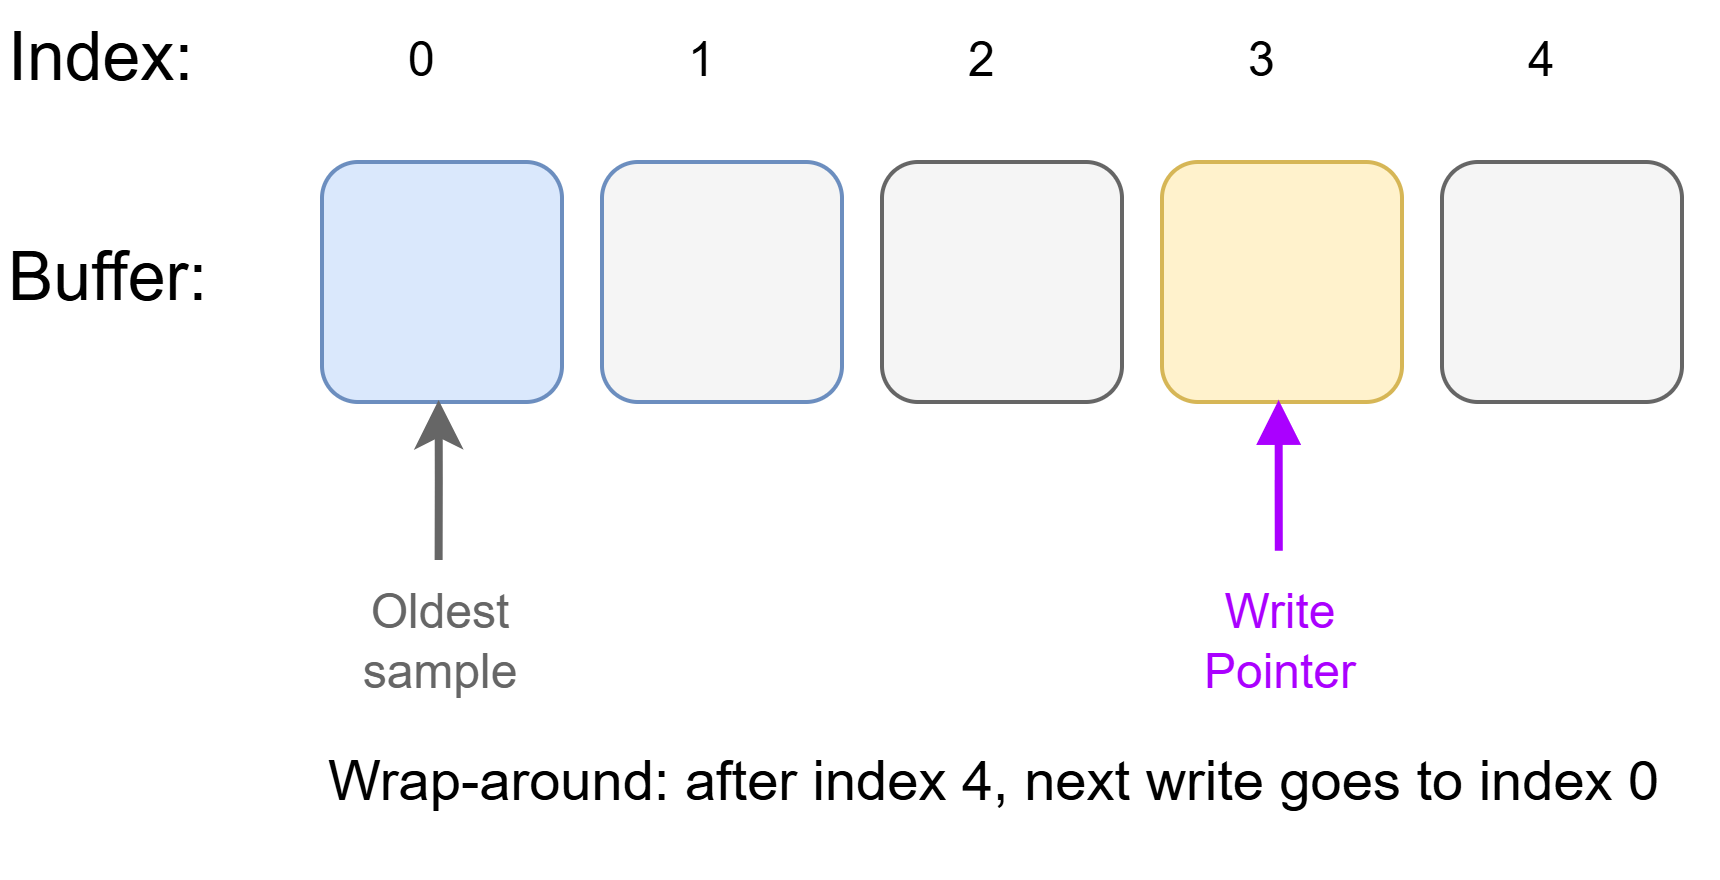
\includegraphics[width=0.7\textwidth]{media/image1.png}
\caption{Illustration of a circular buffer with capacity 5}
\end{figure}

\subsection{Operational
Characteristics}\label{operational-characteristics}

There are two primary operation that ring buffer supports, which are
inserting a new element (push) and removing the oldest element (pop).
The push is going to write data at the current write pointer and then
advances this pointer, but the pop operation different which reads data
from the current read position and advances the read pointer. In the
constant time \(O(1)\), both operation will execute, which is
independent of buffer size, because no data needs to be shifted in
memory.

The buffer has a fixed capacity, defined at compile time. With inserting
elements the number of stored elements will increase till the buffer
going to become full. Once it becomes full the implementation apply the
policy, either block further writes until space becomes available or
overwrite the oldest stored elements as new data arrives. To choose
either block the ring buffer or overwrite is depending on the
requirements of the application, especially with respect to data loss
and real-time constraints.

\subsection{Use Cases in Embedded and Real-Time
Systems}\label{use-cases-in-embedded-and-real-time-systems}

Ring buffers are widely used in embedded and real-time systems because
they provide predictable time behaviour and fixed memory usage. Typical
applications include UART receive buffers, sensor data acquisition
buffers, audio sample queues, and logging mechanisms, where continuous
streams of data must be stored temporarily without dynamic memory
allocation.

In producer--consumer scenarios, such as interrupt-driven input feeding
a slower processing task, the ring buffer decouples the producer and
consumer rates. The producer can store new data as soon as it becomes
available, while the consumer processes data whenever CPU time and
system load permit. This decoupling reduces the risk of data loss due to
short-term timing variations and simplifies the design of real-time data
pipelines.

\section{Ring Buffer in the Measurement Network
Gateway}\label{ring-buffer-in-the-measurement-network-gateway}

This section describes how the ring buffer is used inside the
Measurement Network Gateway. It first explains the functional
requirements and role of the buffer, then presents the concrete data
structure~RingB\_Struct, and finally discusses the timer and
timestamping mechanism that is tightly coupled to the buffer design.

\subsection{2.1 Requirements and Role}\label{requirements-and-role}

In the Measurement Network Gateway, two main threads handle sensor data:

\begin{itemize}
\item
  A~sensor thread~that periodically reads physical sensors (temperature,
  ADC channels, switches, push buttons) and produces timestamped
  samples.
\item
  A~server thread~that packages these samples into TCP payloads and
  transmits them to a remote client.
\end{itemize}

These threads have different timing characteristics. The sensor thread
must respect precise sampling intervals, while the server thread is
constrained by network latency, client behaviour, and the TCP stack. To
decouple these two activities, the gateway requires an intermediate
storage mechanism that:

\begin{itemize}
\item
  Preserves the temporal order of measurements (FIFO behaviour).
\item
  Allows the sensor thread to continue sampling even when the network is
  temporarily slow or unavailable.
\item
  Uses fixed memory to avoid dynamic allocation in an embedded
  environment.
\item
  Supports concurrent access from two threads in a safe manner.
\end{itemize}

The ring buffer serves as a bounded FIFO queue between the sensor thread
(producer) and the server thread(consumer). After the acquisition the
new sample are push to the ring buffer by the sensor thread and the
server thread will pop those samples from rig buffer whenever it is
ready to send data to the client. This design ensures that the sampling
logic is independent of network timing and that the gateway can handle
short bursts of data without losing the most recent measurements.

In this project's implementation, once the buffer is full, new data
overwrites the oldest stored samples. This policy will explain in
details in the next section.

\begin{figure}[H]
\centering 
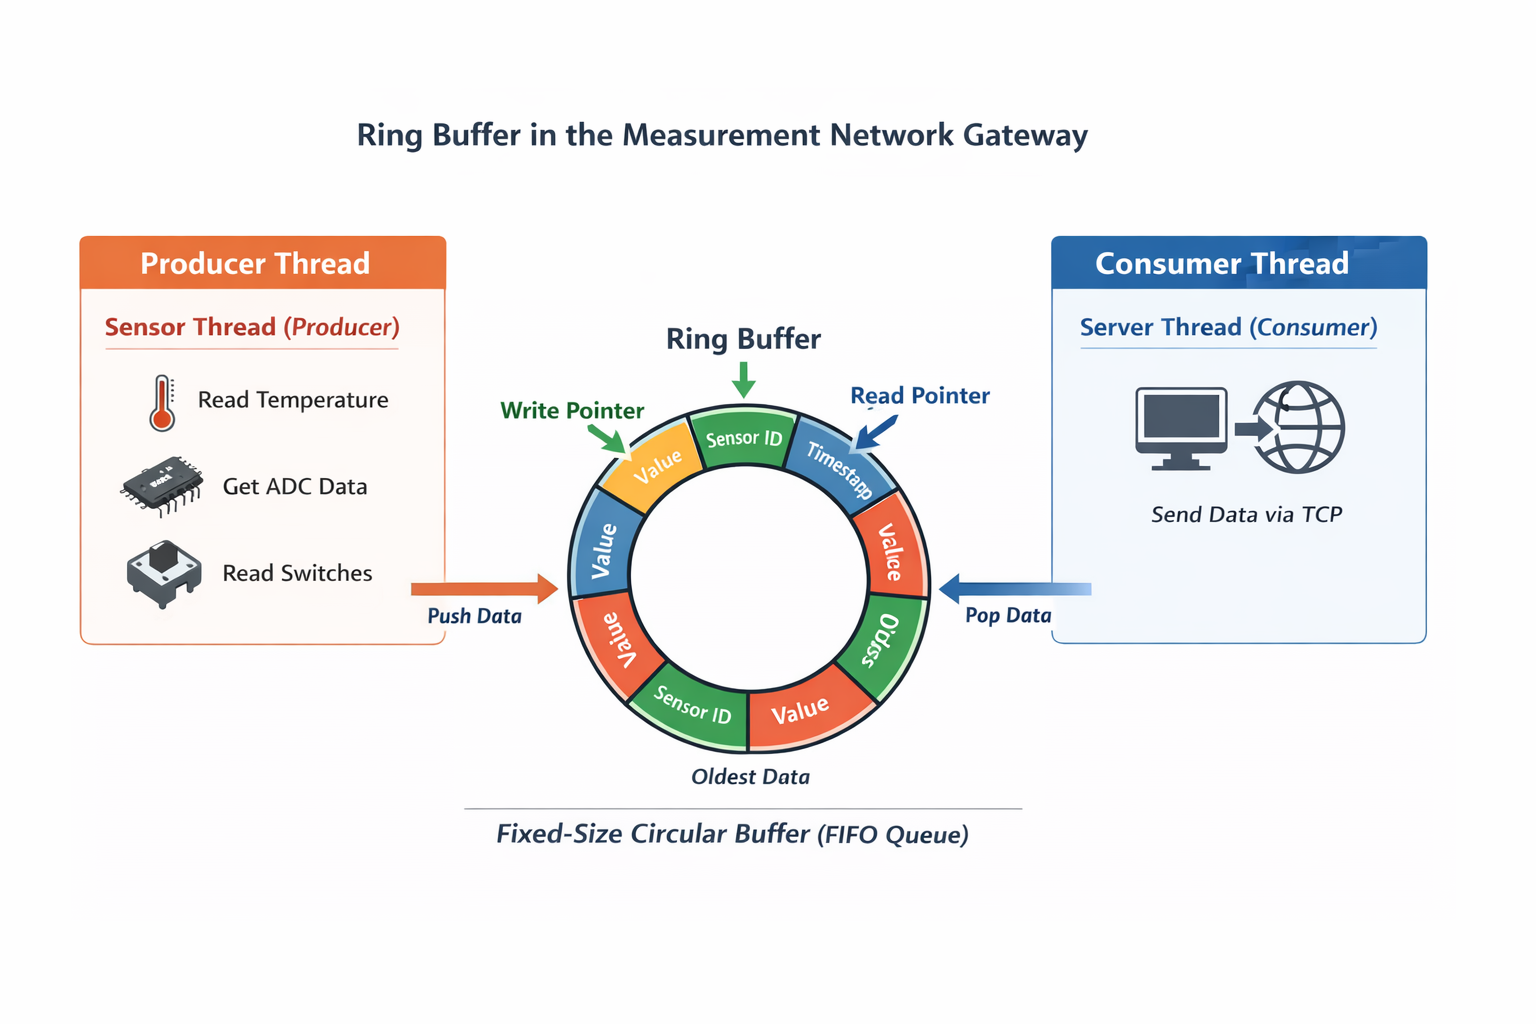
\includegraphics[width = 0.9\textwidth]{media/image2.png}
\caption{Producer–consumer use of the ring buffer.}
\end{figure}

\subsection{Data Structure \texttt{RingB\_Strcut}}
The ring buffer is implemented as a global instance of the structure \texttt{RingB\_Struct}, defined in \texttt{Ring\_Buffer.h}. It groups all storage arrays and control variables needed for FIFO measurement buffering.

\begin{minted}[bgcolor = lightgray, tabsize = 4, breaklines]{c}
#define RBUF_LEN 2048

typedef struct {
    pthread_mutex_t bmutex;              // mutex for thread safety
    volatile int      sensor_id[RBUF_LEN];
    volatile uint64_t tstamp[RBUF_LEN];
    volatile int      svalue[RBUF_LEN];
    volatile int      rb_pointer;        // write index
    volatile int      rb_cnt;            // number of valid entries
} RingB_Struct;

extern RingB_Struct Ring_Buf;
\end{minted}

The fields have the following roles:
\begin{itemize}
\item \texttt{RBUF\_LEN} defines the fixed capacity of the buffer in number of samples (2048 in this project).
\item bmutex protects all accesses to the buffer so that the sensor and server threads cannot modify it at the same time.
\item \texttt{sensor\_id[]}, \texttt{tstamp[]}, and \texttt{svalue[]} are parallel arrays; for any index i, the triple \texttt{(sensor\_id[i], tstamp[i], svalue[i])} represents one complete measurement sample.
\item \texttt{rb\_pointer} points to the position where the next pushed sample will be stored. It is advanced with wrap-around after each write.
\item \texttt{rb\_cnt} stores how many valid samples are currently buffered. It is going to increase on push but decrease on pop. The buffer is full when the \texttt{rb\_cnt} reaches \texttt{RBUF\_LEN} and new samples will overwrite the oldest one while \texttt{rb\_cnt} stays constant.
\end{itemize}
With the storing of the write pointer and a count, the implementation can reconstruct the index of the oldest sample on demand, without the read pointer separated.  This way keeps the state small and also this way will support full FIFO behavior.

\subsection{Timer and Timestamping}
Each measurement in the ring buffer is tagged with a timestamp in microseconds relative to the gateway's startup time. This is implemented in Ring\_Buffer.c using a monotonic system clock.
At startup, the sensor thread calls \texttt{InitTimer()} once to record a reference time:

\begin{minted}[bgcolor = lightgray, tabsize = 4, breaklines]{c}
static uint64_t US_startup_time;

void InitTimer(void)
{
    struct timespec ts;
    clock_gettime(CLOCK_MONOTONIC, &ts);
    US_startup_time = ts.tv_sec * 1000000ULL + ts.tv_nsec / 1000ULL;
}
\end{minted}

Whenever a sensor value is acquired, the thread calls \texttt{GetElapsedTime()} to obtain the current timestamp:

\begin{minted}[bgcolor = lightgray, tabsize = 4, breaklines]{c}
static uint64_t US_startup_time;

void InitTimer(void)
{
    struct timespec ts;
    clock_gettime(CLOCK_MONOTONIC, &ts);
    US_startup_time = ts.tv_sec * 1000000ULL + ts.tv_nsec / 1000ULL;
}
\end{minted}

In this way:
\begin{itemize}
\item InitTimer records a fixed reference time US\_startup\_time in microseconds, using CLOCK\_MONOTONIC, which is not affected by wall clock changes.
\item GetElapsedTime returns the elapsed time since startup, also in microseconds.
\item The sensor thread passes this value as the timestamp parameter of \texttt{PushRB}, so each ring buffer entry contains a time stamp consistent across all sensors.
\end{itemize}
This scheme allows the client to reconstruct the exact timing of measurements and to align data from different sensors on a common time axis.

\section{Implementation Details}
This section explains how the ring buffer is brought into a defined initial state and how measurements are inserted and removed. It covers the initialization functions \texttt{InitTimer} and \texttt{InitRingBuffer}, followed by the \texttt{PushRB} and \texttt{PopRB} operations that implement the FIFO behaviour.

\subsection{Initialization (\texttt{InitTimer}, \texttt{InitRingBuffer})}
The initialization phase prepares both the time base for timestamps and the ring buffer storage. \texttt{InitTimer} was introduced in Section 2.3; it records the startup time using the monotonic system clock and is called once by the sensor thread.

The function \texttt{InitRingBuffer} brings the buffer into a defined empty state:
\begin{minted}[bgcolor = lightgray, tabsize = 4, breaklines]{c}
void InitRingBuffer(void)
{
    pthread_mutex_init(&Ring_Buf.bmutex, NULL);

    Ring_Buf.rb_pointer = 0;
    Ring_Buf.rb_cnt     = 0;

    for (int i = 0; i < RBUF_LEN; i++) {
        Ring_Buf.sensor_id[i] = 0;
        Ring_Buf.svalue[i]    = 0;
        Ring_Buf.tstamp[i]    = 0;
    }
}
\end{minted}
This performs three steps:
\begin{itemize}
\item Initializes the mutex bmutex, enabling safe concurrent access from the sensor and server threads.
\item Sets \texttt{rb\_pointer = 0} and \texttt{rb\_cnt = 0}, marking the buffer as empty and indicating that the first write will occur at index 0.
\item Clears all entries in \texttt{sensor\_id}, \texttt{svalue}, and \texttt{tstamp} to a known state, which simplifies debugging and guarantees deterministic start up behaviour.
\end{itemize}
After \texttt{InitTimer} and \texttt{InitRingBuffer} have been called, the gateway has a clean time reference and an empty, ready to use ring buffer.


\subsection{Push Operation (\texttt{PushRB})}
The function \texttt{PushRB} inserts a new measurement sample into the ring buffer. It is called by the sensor thread whenever a sensor value is acquired.

\begin{minted}[bgcolor = lightgray, tabsize = 4, breaklines]{c}
void PushRB(int sid, uint64_t ts, int sv)
{
    pthread_mutex_lock(&Ring_Buf.bmutex);

    Ring_Buf.sensor_id[Ring_Buf.rb_pointer] = sid;
    Ring_Buf.tstamp[Ring_Buf.rb_pointer]    = ts;
    Ring_Buf.svalue[Ring_Buf.rb_pointer]    = sv;

    if (Ring_Buf.rb_cnt < RBUF_LEN) {
        Ring_Buf.rb_cnt++;
    }

    Ring_Buf.rb_pointer = (Ring_Buf.rb_pointer + 1) % RBUF_LEN;

    pthread_mutex_unlock(&Ring_Buf.bmutex);
}
\end{minted}
The behaviour is as follows:
\begin{itemize}
\item The mutex bmutex is locked to ensure exclusive access to the buffer state during the update.
\item The triple (sid, ts, sv) is written at index \texttt{rb\_pointer}, forming one complete measurement sample.
\item If the buffer is not yet full \texttt{(rb\_cnt < RBUF\_LEN)}, the count of valid entries is incremented; otherwise it remains at \texttt{RBUF\_LEN}, and the oldest sample will later be overwritten.
\item The write pointer \texttt{rb\_pointer} is advanced and wrapped around using modulo arithmetic, implementing the circular structure.
\item Finally, the mutex is unlocked so that other threads can access the buffer again.
\end{itemize}
Conceptually, each call to \texttt{PushRB} appends one new sample to the logical end of the FIFO queue. When the producer is faster than the consumer and the buffer becomes full, new pushes overwrite the oldest data while always preserving the most recent measurements.

\subsection{Pop Operation \texttt{PopRB}}
The \texttt{PopRB} function removes the oldest available sample from the ring buffer and returns it to the caller. It is typically used by the server thread when it prepares a data packet to send to the client.

\begin{minted}[bgcolor = lightgray, tabsize = 4, breaklines]{c}
int PopRB(int *sid, uint64_t *ts, int *sv)
{
    pthread_mutex_lock(&Ring_Buf.bmutex);

    if (Ring_Buf.rb_cnt == 0) {
        pthread_mutex_unlock(&Ring_Buf.bmutex);
        return -1;                      // buffer empty
    }

    int idx = (Ring_Buf.rb_pointer - Ring_Buf.rb_cnt + RBUF_LEN) % RBUF_LEN;

    *sid = Ring_Buf.sensor_id[idx];
    *ts  = Ring_Buf.tstamp[idx];
    *sv  = Ring_Buf.svalue[idx];
    Ring_Buf.rb_cnt--;

    pthread_mutex_unlock(&Ring_Buf.bmutex);
    return 0;                           // success
}
\end{minted}

The steps are:
\begin{itemize}
	\item The mutex is locked to protect the shared state.
	\item If \texttt{rb\_cnt} is zero, the buffer is empty, the mutex is unlocked and -1 is returned to signal “no data available”.
	\item Otherwise, the index of the oldest sample is computed as
\texttt{idx = (rb\_pointer-rb\_cnt+RBUF\_LEN) mod RBUF\_LEN}
which moves \texttt{rb\_cnt} positions back from the next write position, with wrap around.
	\item The sensor ID, timestamp, and value at index idx are copied into the caller’s output parameters, and rb\_cnt is decremented to reflect that one entry has been removed.
	\item Finally, the mutex is unlocked and the function returns 0 to indicate success.
\end{itemize}

\textbf{Example}: Computing the Oldest Sample Index. 
To illustrate the index calculation:
\begin{center}
\texttt{idx = (rb\_pointer-rb\_cnt+RBUF\_LEN) mod RBUF\_LEN}
\end{center}
consider a small ring buffer with \texttt{RBUF\_LEN = 5}. Assume the following state:
Given the following ring buffer state:
\begin{itemize}
    \item $\texttt{RBUF\_LEN} = 5$
    \item $\texttt{rb\_pointer} = 2$ (next write will go to index 2)
    \item $\texttt{rb\_cnt} = 3$ (three valid samples stored)
\end{itemize}

The last three writes have filled three positions immediately before
\texttt{rb\_pointer} in the circular sense. The valid entries are therefore
at indices:
\begin{itemize}
    \item index 4 \quad (oldest sample)
    \item index 0
    \item index 1 \quad (newest sample)
\end{itemize}

The \texttt{PopRB} function must locate the oldest sample, which is at index~4.
Using the formula:
\[
    \texttt{idx} = (\texttt{rb\_pointer} - \texttt{rb\_cnt} + \texttt{RBUF\_LEN})
                  \;\%\; \texttt{RBUF\_LEN}
                = (2 - 3 + 5) \;\%\; 5 = 4
\]

So $\texttt{idx} = 4$, exactly the index of the oldest stored entry. After
\texttt{PopRB} reads the sample at index~4 and decrements \texttt{rb\_cnt}
to 2, the remaining valid samples are at indices~0 and~1, and a subsequent
call with the updated state will correctly return index~0 as the next oldest
entry.

\section{Runtime Data Flow and System Architecture}
This chapter describes the runtime behavior of the Measurement Network Gateway and explains how measurement data flows through the system from hardware acquisition to remote visualization. Rather than focusing on individual hardware devices or data structures in isolation, this chapter presents a system-level view of how threads, timing, and buffering interact during operation.

\subsection{	Thread Architecture Overview}
The Measurement Network Gateway is built around a small multithreaded architecture that separates sensor acquisition from network communication. Two main threads are used in conjunction with a shared ring buffer to transport measurement data to a remote client.

The sensor thread is responsible for interacting with the hardware. It periodically samples physical sensors, generates timestamps, and inserts measurement records into the ring buffer. This thread acts as the producer of measurement data and operates independently of network conditions or client behavior.

The server thread functions as the consumer. It retrieves measurement entries from the ring buffer and transmits them to a remote GUI or client application using a TCP connection. By decoupling the server thread from direct hardware access, the system ensures that temporary network delays do not directly interfere with sensor sampling.

At a high level, the runtime data path through the system is:

\begin{figure}[H]
\centering 
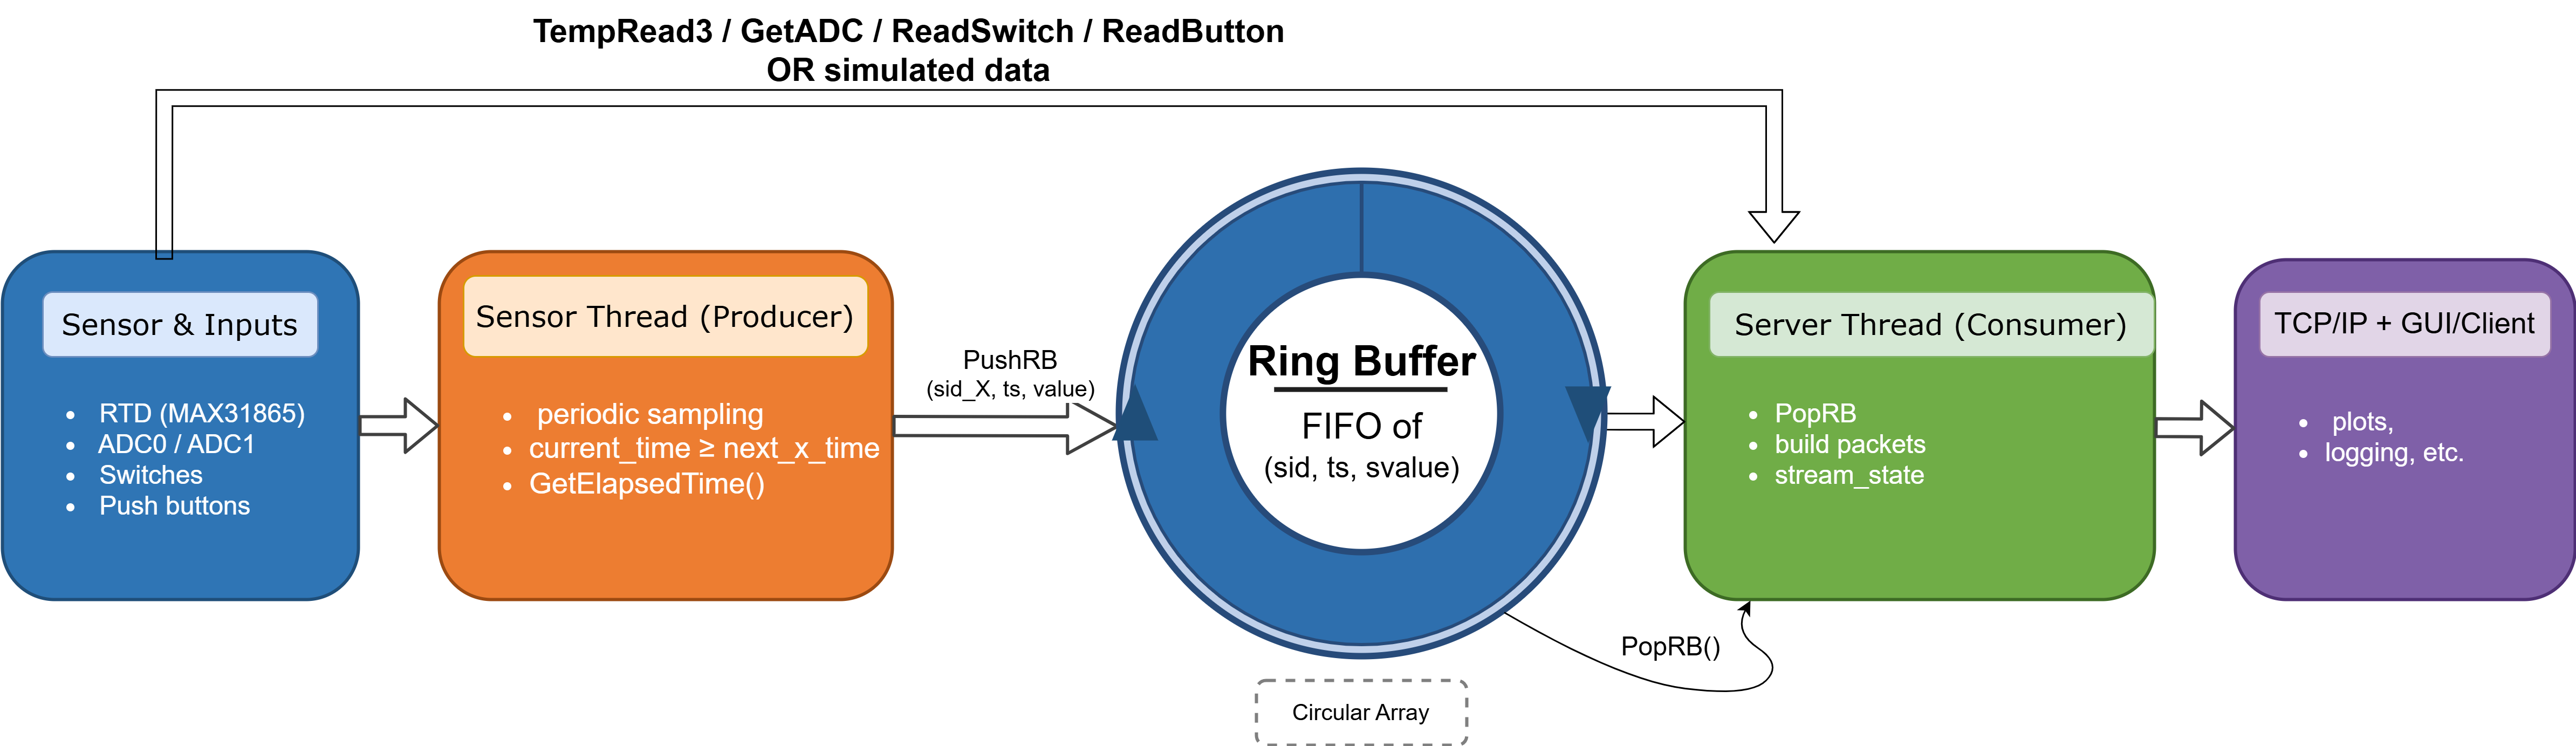
\includegraphics[width = \textwidth]{media/image3.png}
\caption{Runtime data flow of the Measurement Network Gateway}
\end{figure}
This architecture provides a clear separation of concerns and allows each subsystem to operate at its own pace.

\subsection{Producer-Consumer Model}
The ring buffer is acting like a bridge between the sensor thread and the server thread which follows  a classical producer–consumer model implemented. Sensor thread read data or measure the samples and then inserts them into ring buffer, while server thread consumes those samples and sends to the client. 

On the producer side, sensor is sampled each time and then the result is written into the ring buffer using the unified insertion function:

\begin{minted}[bgcolor = lightgray, tabsize = 4, breaklines]{c}
PushRB(sid_temp, current_time, temp_data);
PushRB(sid_adc0, current_time, adc0_data);
PushRB(sid_switches, current_time, switches_data);
\end{minted}

The \texttt{PushRB()} function encapsulates the ring buffer write operation. Internally, it writes a structured entry containing the sensor identifier, timestamp, and value into the current head position and advances the head index. If the buffer is already full, the oldest entry is overwritten by advancing the tail index according to the overwrite policy.

A simplified conceptual form of the write operation is:

\begin{minted}[bgcolor = lightgray, tabsize = 4, breaklines]{c}
rbuf[head].sensor_id = sid;
rbuf[head].tstamp    = timestamp;
rbuf[head].svalue    = value;

head = (head + 1) % RBUF_LEN;

if (head == tail) {
    tail = (tail + 1) % RBUF_LEN;   // overwrite oldest
}
\end{minted}
On the consumer side, the server thread retrieves entries from the ring buffer before sending them over TCP. The read operation removes the oldest available entry and advances the tail index:

\begin{minted}[bgcolor = lightgray, tabsize = 4, breaklines]{c}
if (PopRB(&entry) == 0) {
    send(client_socket, &entry, sizeof(entry), 0);
}
\end{minted}

Here, \texttt{PopRB()} copies the oldest buffered measurement into a local structure and updates the tail pointer. If the buffer is empty, no data is transmitted during that iteration.
Because both threads access shared indices and buffer memory, appropriate synchronization mechanisms are used to ensure consistency. The ring buffer therefore acts as a controlled exchange boundary between acquisition and communication subsystems.

This design allows the producer and consumer to operate asynchronously. The sensor thread maintains deterministic sampling timing, while the server thread operates according to network conditions. The ring buffer absorbs short-term rate mismatches and enforces the overwrite-on-full policy described later. 

\subsection{Timing and Scheduling Strategy}
Sensor sampling is controlled by time based scheduling mechanism which implemented within sensor thread. With initialization, a reference timer is started \texttt{InitTimer}, and elapsed time is subsequently obtained using \texttt{GetElapsedTime}. All timestamps are in microseconds related to system startup. 

The sensor thread maintains an independent next sampling deadline for the each sensor channel. While execution time, the current elapsed time is compared against each channel’s scheduled sampling time using conditions of the form \texttt{current\_time >= next\_x\_time}. If the condition is met, the sensor is sampled and the result is pushed into the ring buffer.

With this procedure, each sensor operate its own sampling frequency while sharing a single execution thread. Microsecond-resolution timestamps enable precise sampling and minimize jitter, particularly when multiple sensors operate at different rates. The timestamp method is much more better than blocking delays which maintains predictable timing behavior and efficient CPU utilization.


\section{Per-Sensor Mapping into the Ring Buffer}
This chapter describes how each physical hardware channel is represented inside the ring buffer. While previous chapters explained the hardware interfaces and the buffer mechanism independently, this section connects the two perspectives. It answers a central architectural question: how does each real-world signal appear as a structured entry in the shared ring buffer?

\subsection{	Sensor ID Enumeration}
To distinguish between different hardware sources within a unified buffer structure, each sensor channel is assigned a unique identifier using the following enumeration:

\begin{minted}[bgcolor = lightgray, tabsize = 4, breaklines]{c}
typedef enum
{
    sid_temp     = 1,
    sid_adc0     = 2,
    sid_adc1     = 3,
    sid_switches = 4,
    sid_pushb    = 5
} sensor_id;
\end{minted}
The \texttt{sensor\_id} value is stored in every ring buffer entry and encodes the origin of the measurement. Because the ring buffer stores heterogeneous data from multiple hardware channels in a single FIFO structure, this identifier is essential for interpreting the stored value correctly.

The consumer side, also server thread and the GUI are using the \texttt{sid} field to interpret the corresponding \texttt{svalue} . Based on the sensor ID the value can be a raw ADC count, a scaled temperature value, or a digital bitfield. This method can keep ring buffer on uniform way while still preserving the semantic meaning of each hardware signal.

\begin{figure}[H]
\centering 
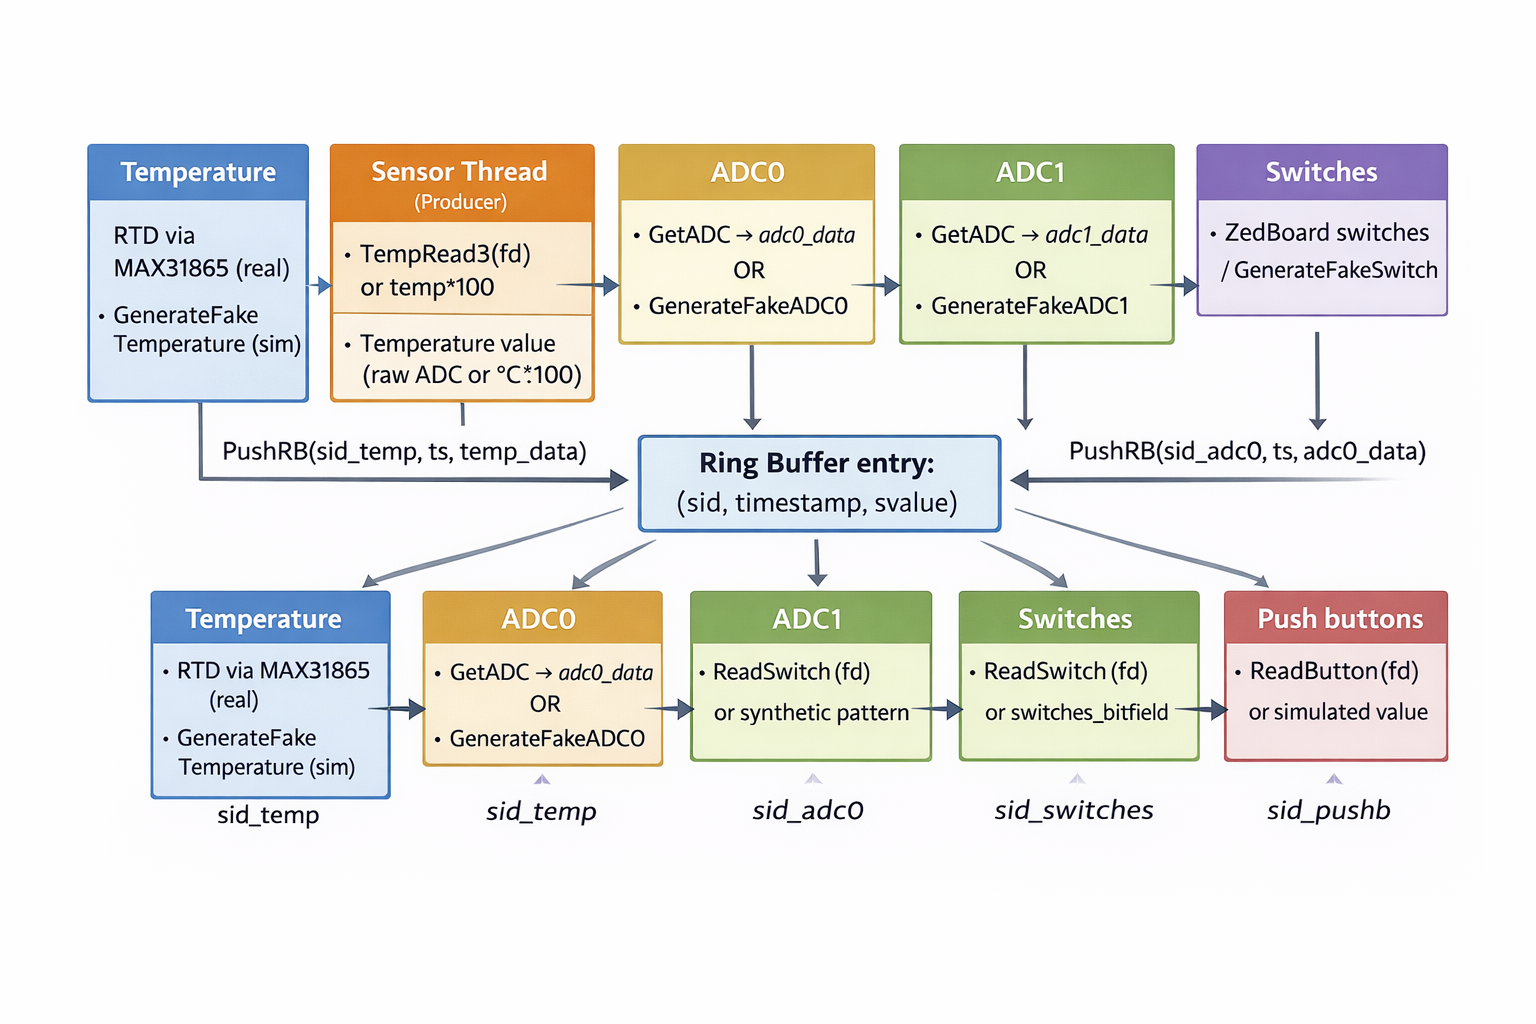
\includegraphics[width = 0.8\textwidth, trim = 0cm 2cm 0cm 0cm, clip]{media/image4.png}
\caption{Per sensor mapping into the ring buffer}
\label{fig-image4}
\end{figure}

The mapping between sensor IDs and hardware sources is summarized below:
\begin{table}[h]
    \centering
    \begin{tabular}{|c|l|l|l|}
        \hline
        \textbf{SID Value} & \textbf{Enum Name} & \textbf{Hardware Source} & \textbf{Typical Units} \\
        \hline
        1 & \texttt{sid\_temp}     & MAX31865 RTD input      & raw ADC code / \textdegree C \\
        2 & \texttt{sid\_adc0}     & ADC channel 0           & raw ADC counts \\
        3 & \texttt{sid\_adc1}     & ADC channel 1           & raw ADC counts \\
        4 & \texttt{sid\_switches} & ZedBoard switches       & 8-bit bitfield \\
        5 & \texttt{sid\_pushb}    & ZedBoard pushbuttons    & 5-bit bitfield \\
        \hline
    \end{tabular}
    \caption{Sensor ID encoding used in the ring buffer}
    \label{tab:sid_values}
\end{table}
This enumeration provides the logical bridge between physical hardware and abstract data records.

\subsection{Temperature Data Path into the Ring Buffer}
The temperature channel follows a time-driven acquisition model within the sensor thread:

\begin{minted}[bgcolor = lightgray, tabsize = 4, breaklines]{c}
if (current_time >= next_temp_time) {
    uint32_t temp_data;
    if (simulation) {
        double temp = GenerateFakeTemperature(current_time);
        temp_data = (uint32_t)(temp * 100);
    } else {
        temp_data = TempRead3(fd);
    }

    PushRB(sid_temp, current_time, temp_data);
    next_temp_time += period_temp_us;
}
\end{minted}
If we look to the hardware side, the temperature measurement is based on the RTD sensor which is connected to the MAX31865 resistance-to-digital converter. The \texttt{TempRead3(fd)} function reads the device via the sensor layer and returns the corresponding ADC value for the RTD resistance. This raw value corresponds directly to the temperature measurement described in the hardware chapter.

In simulation mode, the hardware access is replaced by \texttt{GenerateFakeTemperature()}, which produces a synthetic temperature in degrees Celsius. The value is multiplied by 100 before storage to preserve two decimal places using integer representation.

Regardless of whether the value originates from real hardware or simulation, the final operation is:
\begin{minted}[bgcolor = lightgray, tabsize = 4, breaklines]{c}
PushRB(sid_temp, current_time, temp_data);
\end{minted}
The ring buffer therefore stores a record containing:

\begin{itemize}
\item \texttt{sensor\_id} = sid\_temp
\item \texttt{tstamp} = current\_time (us since startup)
\item \texttt{svalue} = temp\_data (raw ADC or \SI{100}{\degreeCelsius})
\end{itemize}
This unified insertion ensures that downstream components remain independent of the acquisition mode.

\subsection{ADC0 and ADC1 Data Path into the Ring Buffer}
The ADC channels are sampled using similar time-based logic:

\begin{minted}[bgcolor = lightgray, tabsize = 4, breaklines]{c}
PushRB(sid_temp, current_time, temp_data);if (current_time >= next_adc0_time) {
    if (simulation) {
        double dt_adc0 = 1.0 / main_config.adc0_config;
        t_adc0 += dt_adc0;
        adc0_data = (uint32_t)(fake_state.adc0_base
                     + 100.0 * sin(2.0 * PI * freq_adc0 * t_adc0));
    } else {
        GetADC(fd, &adc0_data, &dummy0);
    }
    PushRB(sid_adc0, current_time, adc0_data);
    next_adc0_time += period_adc0_us;
}
\end{minted}
On the hardware side, both \texttt{ADC0} and \texttt{ADC1} are provided by a shared ADC subsystem. The \texttt{GetADC()} function retrieves a combined conversion result from the FPGA/ADC hardware and separates the values corresponding to the two analog channels.

 Although they share physical conversion hardware, they represent distinct electrical input channels.
In simulation mode, synthetic waveforms are generated independently for each channel. ADC0 and ADC1 can therefore exhibit different amplitudes and frequencies, allowing controlled testing of signal behavior.

From the ring buffer perspective, these channels are treated as independent data streams. Each insertion uses either \texttt{sid\_adc0} or \texttt{sid\_adc1}, and each channel maintains its own sampling period and timestamp sequence. Even though they share hardware resources, the ring buffer records them as logically separate measurement streams.

\subsection{Switches and Push Buttons Data Path into the Ring Buffer}
Digital input channels follow the same structural pattern:

\begin{minted}[bgcolor = lightgray, tabsize = 4, breaklines]{c}
if (current_time >= next_switch_time) {
    uint8_t switches_data =
        simulation ? GenerateFakeSwitch(current_time)
                   : ReadSwitch(fd);
    PushRB(sid_switches, current_time, switches_data);
    next_switch_time += period_switch_us;
}

if (current_time >= next_pushb_time) {
    uint8_t pushb_data =
        simulation ? GenerateFakePushButton()
                   : ReadButton(fd);
    PushRB(sid_pushb, current_time, pushb_data);
    next_pushb_time += period_pushb_us;
}
\end{minted}
On the hardware side, \texttt{ReadSwitch()} and \texttt{ReadButton()} access digital input registers in which each bit corresponds to a physical switch or push button on the board. The returned value represents a complete bitfield describing the instantaneous state of all inputs.

In simulation mode, equivalent bit patterns are generated to emulate user interaction.
Within the ring buffer, the entire bitfield is stored as a single integer value using \texttt{sid\_switches} or \texttt{sid\_pushb}. The timestamp attached to each entry allows precise reconstruction of when a switch changed state or when a button was pressed. The GUI decodes the individual bits from the stored value to display the status of each physical input.

\section{Configurable Sampling Rates and Ring Buffer Load}
Each sensor channel’s sampling rate can be changed at runtime using the global configuration and the server side \texttt{configure} command. The configuration parameter such as \texttt{temp\_config, adc0\_config, adc1\_config, switch\_config}, and \texttt{pushb\_config }is going to set the sampling frequency for corresponding sensor in samples per second (Hz).

The frequency is converted to the time period which is shown in microseconds and then the sensor thread use this time to schedule acquisitions:

\begin{minted}[bgcolor = lightgray, tabsize = 4, breaklines]{c}
uint64_t period_temp_us   = (main_config.temp_config > 0) ? 1000000ULL / main_config.temp_config : 0;
uint64_t period_adc0_us   = (main_config.adc0_config > 0) ? 1000000ULL / main_config.adc0_config : 0;
uint64_t period_adc1_us   = (main_config.adc1_config > 0) ? 1000000ULL / main_config.adc1_config : 0;
uint64_t period_switch_us = (main_config.switch_config > 0) ? 1000000ULL / main_config.switch_config : 0;
uint64_t period_pushb_us  = (main_config.pushb_config > 0) ? 1000000ULL / main_config.pushb_config : 0;
\end{minted}
A higher configuration value therefore results in a shorter sampling period and more frequent sensor reads. Each completed sampling event produces one new ring buffer entry via PushRB(). As a result, the total rate at which data is inserted into the ring buffer is equal to the sum of the sampling rates of all enabled sensor channels.

The configuration can be modified dynamically by the client using the configure command, which is parsed and applied by the server thread:

\begin{minted}[bgcolor = lightgray, tabsize = 4, breaklines]{c}
else if (!strncmp(receive_command, "configure ", 10)) {
    config_struct config2;
    sscanf(&receive_command[10], "%u %u %u %u %u",
           &config2.temp_config,
           &config2.adc0_config,
           &config2.adc1_config,
           &config2.switch_config,
           &config2.pushb_config);
    set_config(&config2);
}
\end{minted}

Changing these parameters directly affects the load placed on the ring buffer. Higher sampling frequencies increase the number of samples produced per second and therefore reduce the amount of time the buffer can retain historical data before older entries are overwritten. Conversely, lower sampling rates reduce buffer pressure and increase the effective history depth.

Let me explain with an example, if ADC0 samples at 1000 Hz and the temperature sensor at 100 Hz, the sensor thread will add roughly 1100 samples per second to the ring buffer. With a ring buffer length of 2048 entries, this corresponds to roughly 1.8 seconds of stored history before the overwrite-on-full policy begins to discard the oldest samples, assuming the consumer does not keep up.

This relation of configuration and sampling is connecting directly how the ring buffer is working. Sampling rates are a trade-off between time resolution and buffer lifespan, and should be chosen with consumer throughput and buffer capacity in mind.

\section{Simulation vs. Real Hardware with a Unified Ring Buffer API}
The Measurement Network Gateway supports both real hardware operation and a fully functional simulation mode. During initialization, the application attempts to open the device file \texttt{/dev/meascdd} to access the measurement hardware. If this operation fails, the system automatically enables simulation mode by setting the simulation flag to 1. This allows the application to continue running without physical hardware present.

Within the sensor thread, each sensor acquisition branch checks the value of the simulation flag. In real hardware mode, the system calls the corresponding hardware access functions, such as \texttt{TempRead3(), GetADC(), ReadSwitch(),} and \texttt{ReadButton()}. These functions retrieve actual measurement data from the RTD interface, ADC subsystem, or digital input registers.

In simulation mode, the hardware calls are replaced with synthetic data generators. Functions such as \texttt{GenerateFakeTemperature(), GenerateFakeADC0(), GenerateFakeADC1(),} \texttt{GenerateFakeSwitch()}, and \texttt{GenerateFakePushButton()} produce artificial measurement values that emulate realistic sensor behavior. This enables development, testing, and demonstration without requiring the physical hardware platform.

Despite these different acquisition paths, all sensor branches converge at the same interface:
\begin{minted}[bgcolor = lightgray, tabsize = 4, breaklines]{c}
PushRB(sid_X, current_time, value);
\end{minted}
Whether the value is reading from the real hardware or simulated generator are inserted to the ring buffer by the \texttt{PushRB()} function and the same structured data format. There is no difference for the ring buffer that those data are real data or simulated data. Likewise, the server thread retrieves and transmits measurement records without any knowledge of their origin.

This design ensures that the ring buffer and server components form a hardware-agnostic measurement pipeline. The acquisition layer can switch between real and simulated inputs without changing data transport, buffering, or network streaming. This separating concerns boosts modularity, simplifies testing, and strengthens system reliability.

\section{Design Discussion and Trade-Offs}
The ring buffer implementation in the Measurement Network Gateway reflects several conscious design decisions. This section discusses the most important trade-offs: buffer capacity, overwrite behaviour, and synchronization strategy.

\subsection{Buffer Size and Latency}
The capacity \texttt{RBUF\_LEN} is fixed at 2048 samples. A larger buffer lets the system handle longer delays in the server or network, since more data can be queued before old samples are overwritten. There are also some problem with increasing the ring buffer that consumes more memory and also increase the worst-case latency between acquisition and transmission, which cause the sample should wait much longer in the queue before it is sent.

The chosen size represents a compromise between robustness and responsiveness. For the intended measurement use case, it is more important to have some buffering against short network delays than to guarantee that every historical sample is preserved indefinitely. If strict lossless recording over long periods were required, a different design using larger storage or disk logging would be necessary.

\subsection{Overwrite-on-Full Policy}
When \texttt{rb\_cnt} reaches\texttt{ RBUF\_LEN}, the buffer is logically full. In this implementation, \texttt{PushRB} continues to accept new samples: the write pointer advances and the oldest data is implicitly overwritten, while \texttt{rb\_cnt} remains at \texttt{RBUF\_LEN}. This overwrite-on-full policy prioritises the most recent measurements over older ones.

This choice is appropriate for real-time monitoring, where the client typically cares about the current state of the system and a continuous live stream, rather than a complete historical log. Dropping the oldest samples avoids blocking the sensor thread and preserves real-time behaviour even under temporary overload. The trade-off is that, during prolonged overload, some older measurements are lost. An alternative design would block the producer when the buffer is full, which preserves all data but risks disturbing sampling timings or even stalling the measurement process.

\subsection{Synchronization with a Single Mutex}
With the single \texttt{mutex, bmutex} ensures the safety thread and protect all access to the ring buffer. \texttt{PushRB} and \texttt{PopRB} use the same mutex to protect the small section that updates indices and arrays. This is a very simple and easy approach for a dingle producer and single consumer setup, that works well. The both operation push and pop are short and bounded in time.

You could also use lock-free buffers or separate mutexes and condition variables to indicate data or space availability. This kind of approach will reduce blocking and improve scalability in multi-producer or multi-consumer systems, but there is a drawback which is complexity and difficult to verify it. For this gateway, with one sensor thread and one server thread, a single mutex provides deterministic, constant-time operations without introducing significant overhead.

The ring buffer thus provides a deterministic, bounded, and thread-safe mechanism for exchanging data between the acquisition and networking parts of the gateway. The next chapter builds on this buffering layer to describe the sensor-reading implementation and hardware interface in detail.


















%functions for reading the sensors in MNG (Measurement Network Gateway) 

\section{Sensor Readout Module}
The sensor readout logic of the Measurement Network Gateway is encapsulated in the dedicated source file \texttt{sensor\_read.c} with its public interface declared in \texttt{sensor\_read.h}. This module hides all low level details of SPI communication, ADC configuration, and conversion formulas behind a small set of functions that can be called directly from the sensor thread. In this way, the sensor thread only focuses on sampling timing and pushing values into the ring buffer, while \texttt{sensor\_read.c} provides type safe access to the underlying hardware channels.

The most important functions in this module for physical sensor acquisition are:
\begin{itemize}
    \item MAXWrite and MAXRead for low level SPI access to the MAX31865 RTD converter.
    \item TempRead3 (TempRead) for high level temperature measurement in degrees Celsius.
    \item GetADC for sampling generic analog channels via the on board ADC.
\end{itemize}

The following subsections describe each of these functions in turn and illustrate how they are used inside the application code.


\subsection{MAXWrite: writing to MAX31865 registers}
The function \texttt{MAXWrite} is responsible for sending configuration and control data to the MAX31865 temperature sensor interface over the SPI bus. The MAX31865 is a resistance to digital converter (RTD interface) which measures the resistance of a Pt100/Pt1000 sensor and converts it into a digital code that can later be transformed into a temperature value. To operate correctly, the device must be configured by writing specific bits into its configuration register, for example to select 2 wire/3 wire/4 wire mode, enable bias current, set fault thresholds, or start a one shot conversion.
\texttt{MAXWrite} abstracts this SPI write transaction into a single C function call. Internally, it typically performs the following steps:
\begin{itemize}
    \item Asserts the chip select line (CS) of the MAX31865 to start an SPI frame.
    \item Sends the register address ORed with the write bit as the first byte on the SPI bus.
    \item Sends one or more data bytes that contain the configuration or control information.
    \item De asserts the chip select line to complete the transfer.
\end{itemize}

By concentrating all these operations in MAXWrite, the rest of the code never has to deal with the exact SPI timing or bit level format of the MAX31865 registers; it simply calls MAXWrite with the desired register and data.


\subsection{MAXRead: reading from MAX31865 registers}
Complementary to MAXWrite, the function MAXRead performs SPI read operations from the MAX31865. It is used to obtain the current configuration, read status and fault flags, and, most importantly, fetch the raw RTD measurement data from the converter. The raw measurement is typically stored in two consecutive registers, for example MSB and LSB of the RTD code, which must be read in a single SPI transaction and then combined into a 16 bit value.
Internally, MAXRead carries out these steps:
\begin{itemize}
    \item Asserts the chip select line of the MAX31865.
    \item Sends the start register address ORed with the read bit.
    \item Clocks out one or more bytes from the device while sending dummy bytes on MOSI.
    \item De asserts chip select and returns the received bytes to the caller.
\end{itemize}
This design ensures that every place in the code that needs data from the MAX31865 (for example, the raw RTD code or the fault status) can simply call MAXRead with a register address and buffer, without directly manipulating the SPI peripheral.


\subsection{TempRead: high level temperature acquisition}
The function \texttt{TempRead} provides a complete, high level temperature measurement in degrees Celsius, suitable for direct storage in the ring buffer. From the perspective of the sensor thread, \texttt{TempRead} is the only interface needed to acquire the physical temperature; it hides all the intermediate steps such as triggering a conversion, waiting for completion, reading raw codes, and applying calibration or scaling factors.
A typical measurement cycle performed by TempRead3 involves the following stages:
\begin{itemize}
    \item Optionally configure or re configure the MAX31865 using MAXWrite (for example, clear faults or start a one shot conversion).
    \item Wait for the conversion to complete, either by polling a status bit or using a fixed delay sufficient for the conversion time.
    \item Read the raw RTD code from the MAX31865 using MAXRead as shown above.
    \item Convert the raw code into a resistance value and then into a temperature in degrees Celsius according to the transfer function specified in the datasheet.
    \item Return the resulting floating point temperature value to the caller.
\end{itemize}

Because all these details are encapsulated, the rest of the system can treat TempRead3 as a black box that simply returns the current temperature.


\subsection{GetADC: analog to digital conversion}
In addition to the RTD temperature sensor, the Measurement Network Gateway also acquires analog signals via on board ADC channels. These may be used, for example, to measure external sensor voltages, reference levels, or other analog quantities connected to the system. The function GetADC provides a generic interface to read one sample from a specified ADC channel.

GetADC typically takes an integer channel index as an argument and performs the following steps internally:

\begin{itemize}
    \item Selects the appropriate ADC channel in the ADC peripheral registers.
    \item Starts or triggers a conversion on that channel.
    \item Waits until the conversion is complete (polling a status flag or waiting for an interrupt driven result).
    \item Reads the converted digital sample from the ADC data register.
    \item Returns the sample as an integer (for example a 12 bit or 16 bit value) to the caller.
\end{itemize}
By encapsulating this procedure in GetADC, the sensor thread does not need to know any low level details about ADC configuration or status handling; it simply requests a sample from channel 0 or 1 and receives a ready to use digital value.


\subsection{Integration into the overall measurement path}
Together, \texttt{MAXWrite, MAXRead, TempRead3}, and \texttt{GetADC} form the core of the sensor readout path in the Measurement Network Gateway. All physical measurements flow through these functions before being encoded into the abstract ring buffer format used by the rest of the system. The separation between low level driver functions and high level thread logic simplifies both understanding and maintenance of the code:

hardware specific changes (for example, different ADC resolution or a new RTD interface) are localized inside \texttt{sensor\_read.c}, while the sensor thread and server thread can remain unchanged.
